
\documentclass[11pt]{article}
\PassOptionsToPackage{svgnames}{xcolor}
\usepackage{graphicx} % Required for inserting images
\usepackage[utf8]{inputenc}
\usepackage[margin=1in]{geometry}
\usepackage{enumerate, fancyhdr, color, verbatim, setspace, multirow, multicol,subcaption, booktabs, caption, amsfonts}
\usepackage{rotating}
\usepackage{amsmath}
\usepackage{amsthm}
\usepackage{listings}
\numberwithin{equation}{section}

\theoremstyle{definition} 
\newtheorem{definition}{Definition}[subsection]
\newtheorem{theorem}{Theorem}[subsection]
\newtheorem{corollary}{Corollary}[subsection]

\usepackage{colortbl}
\usepackage{tikz}
\usetikzlibrary{matrix, positioning, shadings, shadows}
\usepackage{pgfplots}
\pgfplotsset{compat=1.18}
\usepackage[shortlabels]{enumitem}
% \usepackage[symbol]{footmisc}
\usepackage{multirow}
\usepackage{multicol}
% Creates the header and footer. You can adjust the look and feel of these here.
\usepackage{hyperref}
\hypersetup{
    colorlinks,
    citecolor=black,
    filecolor=black,
    linkcolor=blue,
    urlcolor=blue
}
\newcommand{\bp}{\mathbb{P}}

\definecolor{lightgray}{RGB}{230, 230, 230}
\definecolor{lightgrey}{RGB}{200, 200, 200}

\usepackage{tcolorbox}
\newenvironment{myblock}[1]{%
    \tcolorbox[beamer,%
    noparskip,breakable,
    colback=lightgray,colframe=black,%
    colbacklower=lightgrey,%
    title=#1]}%
    {\endtcolorbox}

\tcbuselibrary{skins,breakable}


\renewcommand{\headrulewidth}{0.2pt} %Creates a horizontal line underneath the header
\setlength{\headheight}{15pt} %Sets enough space for the header
% \renewcommand{\theenumi}{\alph{enumi}}
\onehalfspacing

\usepackage{chngcntr}
\counterwithin{figure}{section}

\DeclareMathOperator*{\argmin}{arg\,min}
\DeclareMathOperator*{\argmax}{arg\,max}

\usepackage[backend=biber, style=authoryear, maxcitenames=2, maxbibnames=9]{biblatex}
\DeclareDelimFormat{nameyeardelim}{\addcomma\space}
\addbibresource{references.bib}

\setcounter{tocdepth}{2}

\title{MGTECON 603 - Questions(Wk 5)\\ (Instructor: Guido Imbens)}
\author{Wooyong Park}
\date{\today}

\begin{document}


\maketitle

This is a document for the questions I had on the fifth week of the course.

\section{Heteroskedasticity-Robust Standard Errors and test-statistic distribution}

\begin{figure}[h]
    \centering
    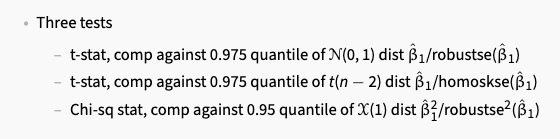
\includegraphics[width=0.7\textwidth]{images/wk5-1.png}
    \caption{Slides 9 page 6}
    \label{fig:slides-9-page-6}
\end{figure}

In figure \ref{fig:slides-9-page-6}, the professor said that the test-statistic distribution does not follow the t-distribution when we use the heteroskedasticity-robust standard errors.

At first, I thought this was because of the heteroskedasticity that the robust standard errors assume, so it's basically a problem with the model assumptions, not the EHW(Eicker-Huber-White) method itself.

I thought that, since EHW standard errors and homoskedastic standard errors are both unbiased and consistent estimators of the variance of the regression coefficient, the test-statistic distribution should follow the same t-distribution.

However, Gemini AI told me the otherwise: 

\begin{tcolorbox}[colback=lightgray, colframe=black, title={Query(Gemini AI):  But even if I use EHW, if the homoskedasticity assumption does hold true, then since EHW is also unbiased estimator of the true standard deviation in that case, wouldn't I still have t-dstibution?}, breakable]
    This is a sharp insight, but unfortunately, no, it still does not follow a t-distribution.
    Here's the simple reason: The t-distribution is a ``family" of distributions. 
    The only reason we get the exact t-distribution in the classical case is that the two components of the t-statistic ($Z$ and $V$) are mathematically perfect and independent:
    \begin{itemize}
        \item Numerator: $Z = \frac{\hat{\beta} - \beta}{\sigma\sqrt{C_{jj}}} \sim N(0,1)$
        \item Denominator: $\sqrt{V/(n-k)} = \sqrt{\frac{(n-k)s^2/\sigma^2}{n-k}} = \frac{s}{\sigma}$
    \end{itemize}
    where $C_{jj} = [(X'X)^{-1}]_{jj}$.
    The proof relies on $s^2$ (the classical variance estimator) being the exact term needed to cancel out the $\sigma$ in the numerator, and $s^2$ itself being based on a $\chi^2$ variable.
    The EHW standard error, $se_{EHW}$, is a completely different formula. 
    Even if homoskedasticity is true, the EHW formula is just a different calculation. 
    When you build the test statistic, the algebra doesn't simplify:
    $$W = \frac{\hat{\beta}_j - \beta_j}{se_{EHW}(\hat{\beta}_j)}$$
    This ratio is no longer a $N(0,1)$ variable divided by the square root of an independent $\chi^2/(n-k)$ variable. It's a ``pseudo" t-statistic or Wald statistic. 
    It doesn't match the precise mathematical definition of a t-distributed random variable.
    Takeaway: The t-distribution is a finite-sample result that requires all classical assumptions, including the specific formula for the standard error. The EHW estimator's value is asymptotic consistency (it's right on average in large samples), not finite-sample exactness.
\end{tcolorbox}

Here, I understand that the numerator and the denominator of the test statistic directly follow the Student's theorem when we have homoskedasticity.
However, I still do have a hunch that the test statistic could follow the t-distribution in any way. I want to know something, or some resource, which directly negates this hunch.

\section{Multiple Coefficients Case($\chi^2$ vs $F$ distribution)}

\begin{figure}[h]
    \centering
    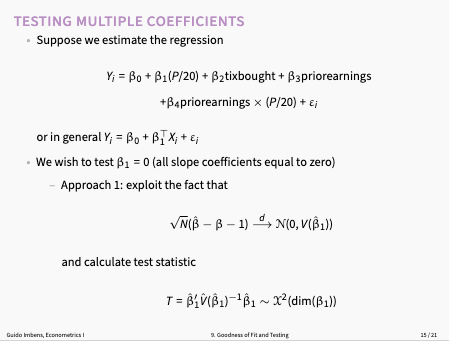
\includegraphics[width=0.5\textwidth]{images/wk5-2.png}
    \caption{Slides 9 page 15}
    \label{fig:slides-9-page-15}
\end{figure}

In slide \ref{fig:slides-9-page-15}, we see that the quadratic form statistic follows the $\chi^2$ distribution when we have multiple coefficients.
This directly corresponds to the univariate case, where the squared t-statistic asymptotically follows the $\chi^2$ distribution, since the t-statistic itself asymptoticallyfollows the standard normal distribution.
But when we have \textbf{normality and the homoskedasticity assumptions regarding the error term}, the squared t-statistic exactly follows the $F$ distribution.

I wonder if the same happens to this multivariate case. Would the quadratic form statistic follow the $F$ distribution, if we have the normality and the homoskedasticity assumptions regarding the error term?


\subsection{Approach 2: run unrestricted and restricted regressions}

\begin{figure}[h]
    \centering
    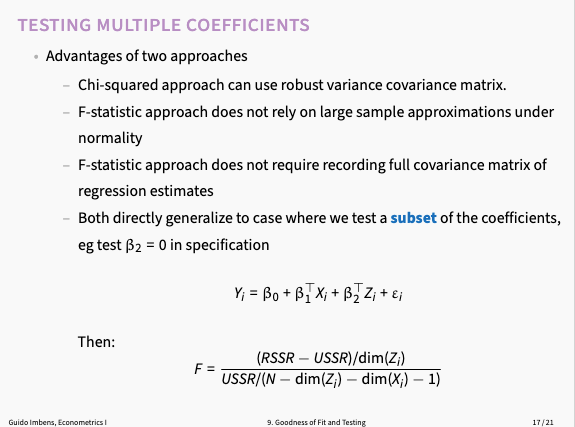
\includegraphics[width=0.5\textwidth]{images/wk5-3.png}
    \caption{Slides 9 page 16}
    \label{fig:slides-9-page-16}
\end{figure}

In slide \ref{fig:slides-9-page-16}, we see that we can do a F-test using the mean squared errors fromf the unrestricted and restricted regressions.
Would this still implicitly assume the normality and the homoskedasticity assumptions regarding the error term?


These are all the questions I had on the fifth week of the course.
I appreciate your help and detailed explanations throughout the course. Many thanks!

\end{document}
